\section{Problem B - SDMA aspect}
\textit{Use the defined antenna patterns/directional signals from exercise A . You would need also some results/idea about exercise A2, if not finished (remember two main tasks : one to find C/I with directional spread signals, other to find shape of full radar sweep (effective antenna pattern wrt user and interferer) and resulting mean direction)}

\subsection{Question 1}
\textit{Now consider a 120 degree sector serviced with above antenna pattern in a SDMA operation (i.e. identical but offset patterns for N users). Consider the system to have power control so all users have same power received at the BS when the individual users antenna pattern maximum is pointed to their respective direction. Assume only a single path from user to BS (like exercise A1))}

\subsubsection{a) For a target C/I=9dB (spatial interference), what is the required user-to-interferer offset angle (to left and right)?. If C/I is 15 dB what then?}

\begin{figure}[!h]
  \centering
  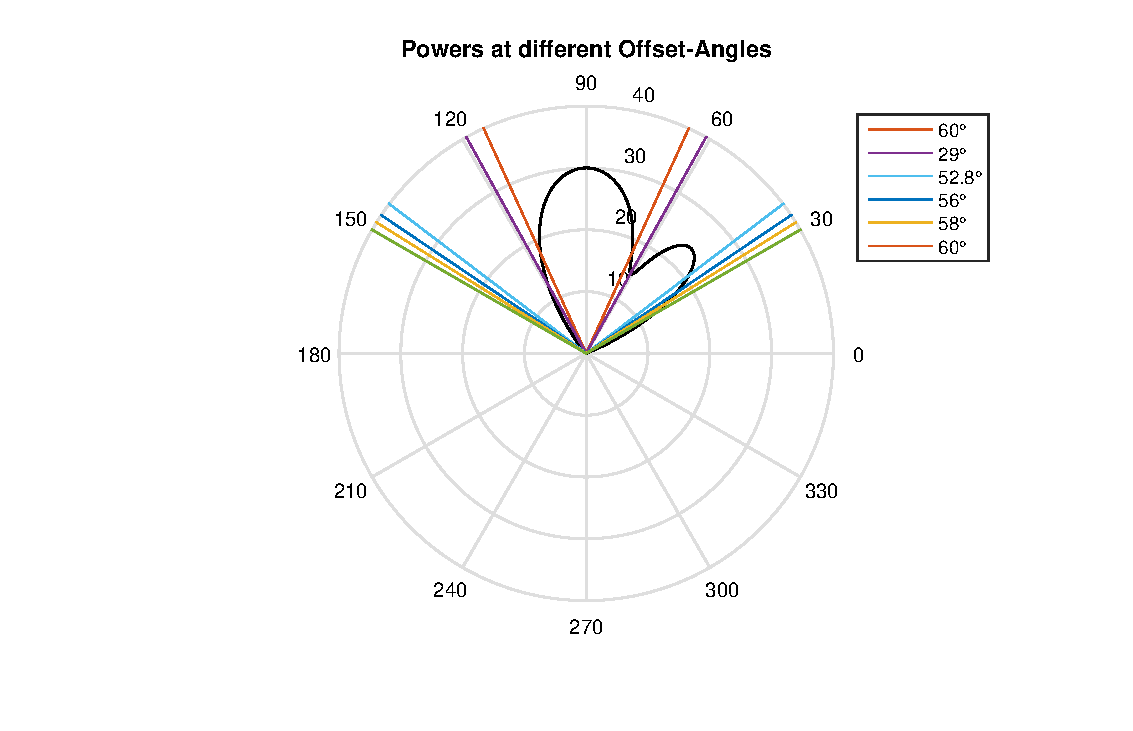
\includegraphics[width=12cm]{offset_angles.eps}
  \caption{Offset angles.}
  \label{fig:offset_angles}
\end{figure}

\begin{figure}[!h]
  \centering
  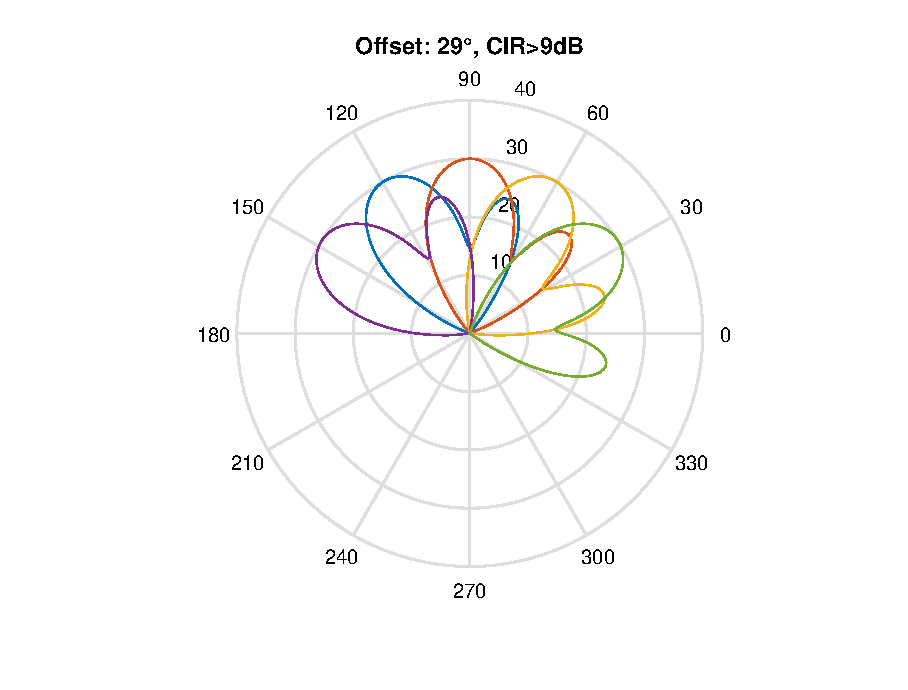
\includegraphics[width=11cm]{offset29deg.eps}
  \caption{Offset 29deg.}
  \label{fig:offset29deg}
\end{figure}

\begin{figure}[!h]
  \centering
  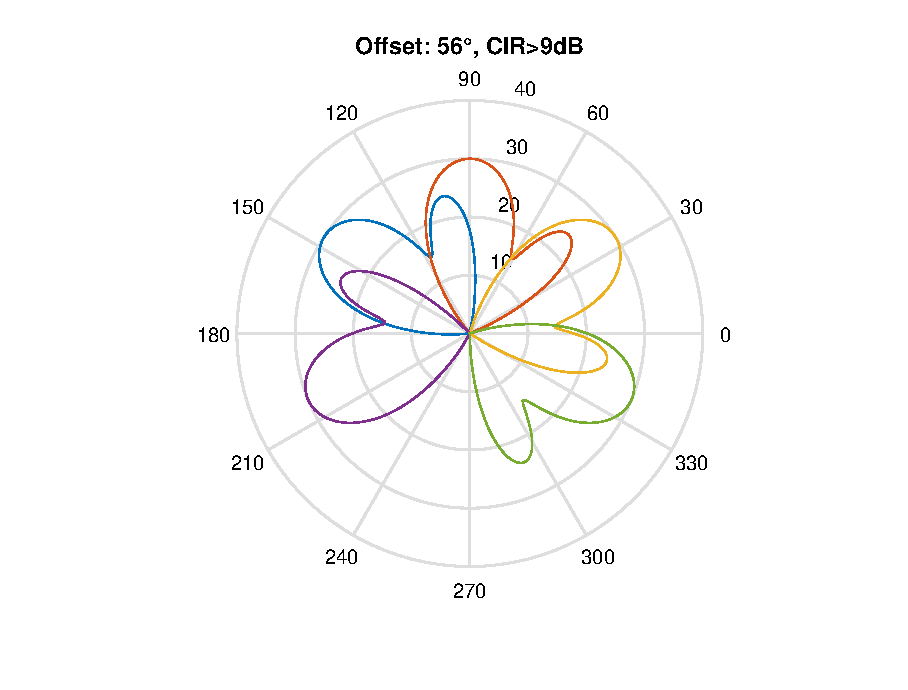
\includegraphics[width=11cm]{offset56deg.eps}
  \caption{Offset 56deg.}
  \label{fig:offset56deg}
\end{figure}

\begin{figure}[!h]
  \centering
  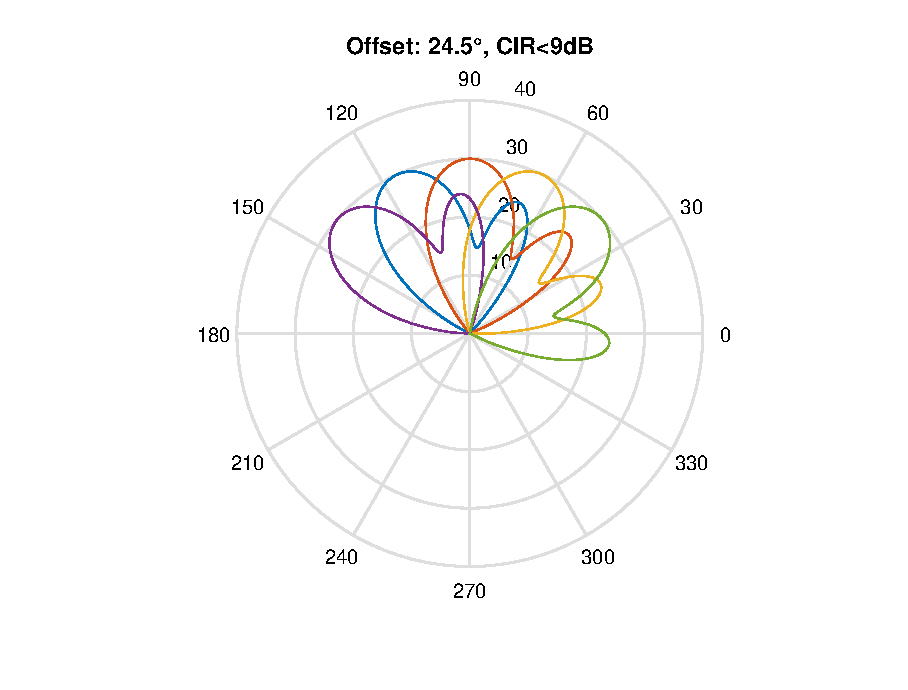
\includegraphics[width=11cm]{offset245deg.eps}
  \caption{Offset 24.5deg.}
  \label{fig:offset245deg}
\end{figure}

\begin{figure}[!h]
  \centering
  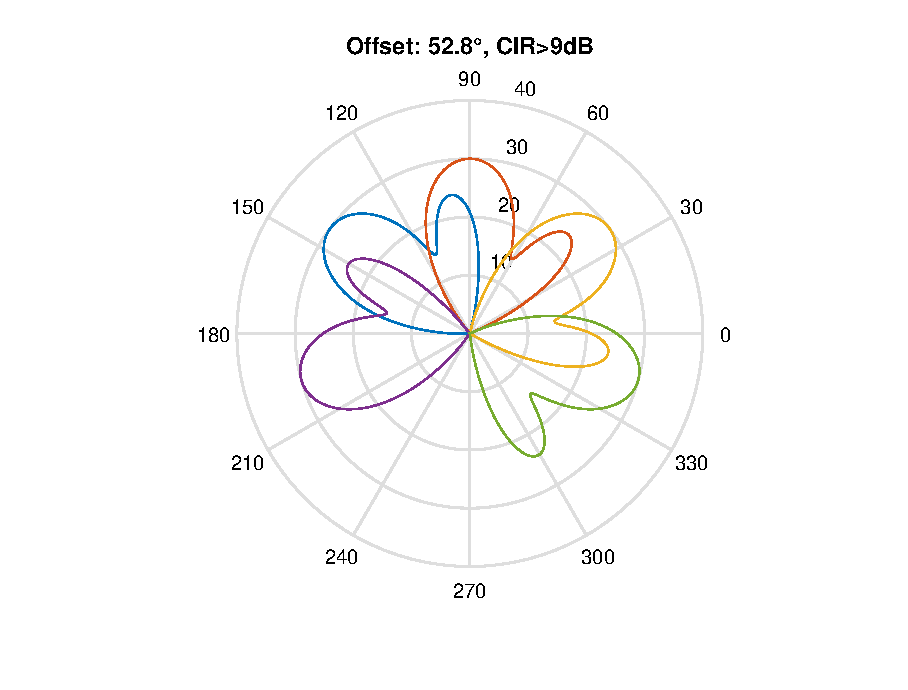
\includegraphics[width=11cm]{offset528deg.eps}
  \caption{Offset 52.8deg.}
  \label{fig:offset528deg}
\end{figure}

\begin{figure}[!h]
  \centering
  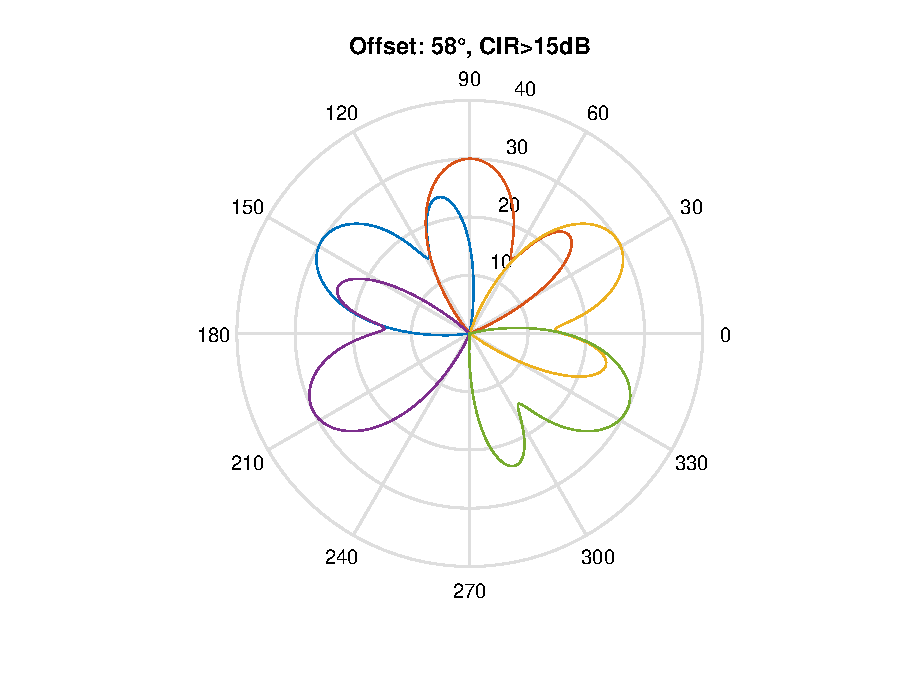
\includegraphics[width=11cm]{offset58deg.eps}
  \caption{Offset 58deg.}
  \label{fig:offset58deg}
\end{figure}

\begin{figure}[!h]
  \centering
  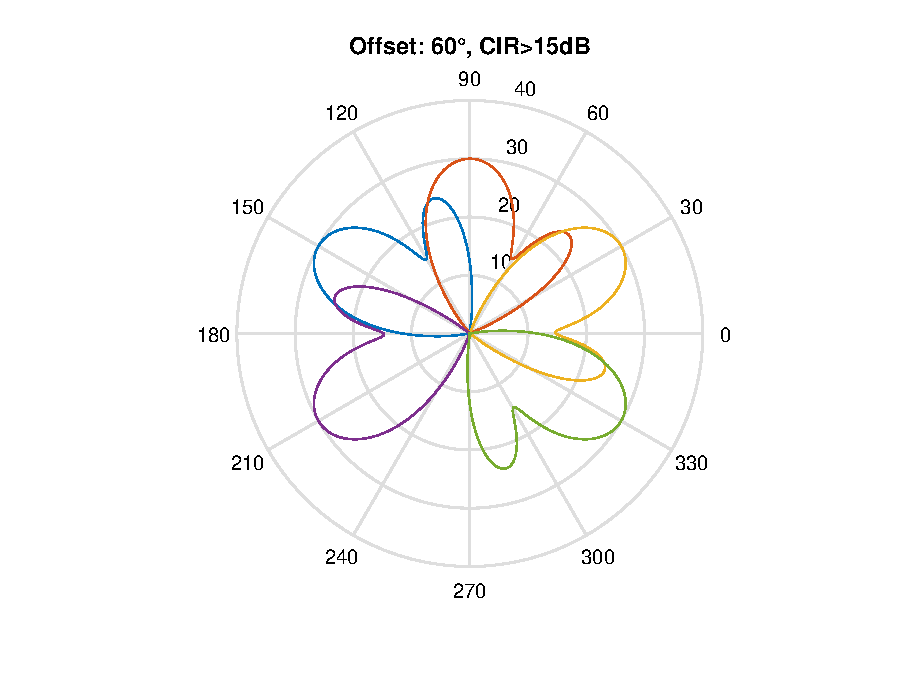
\includegraphics[width=11cm]{offset60deg.eps}
  \caption{Offset 60deg.}
  \label{fig:offset60deg}
\end{figure}

\subsubsection{b) How many spatially separated users can be served in the sector, under the conditions mentioned in a)?. I.e. what is N=?}


\subsection{Question 2}
\textit{Exchange the single path connections in exercise 1, to an angular uniform distribution over 20degree span and with a power density of 1 (similar to Cs in exercise A2). What changes result in the questions 1a) and 1b)?}
